\chapter{Field-based Distributed State Estimation}
\label{ch:distributed-state-estimation}

Cooperation in a collective adaptive system requires devices 
 to combine information that no individual device can obtain alone.
%
In cooperative learning, 
 this information takes the form of distributed data, 
 model updates, or interaction experience.
%
A complementary problem is to reconstruct the current state 
 of the environment from partial and noisy observations.
%
Both problems require an organization of information exchange that remains meaningful when communication is local 
 and device availability changes.
%
This chapter investigates this coordination problem through distributed state estimation, 
 extending the thesis perspective from learning mechanisms to the collective perception that can support adaptive behavior.

The contribution combines a field-based formulation of \gls{DPF}~\cite{DBLP:journals/corr/abs-2606-18483} 
 with its extension to multi-target tracking and mobile sensing~\cite{DBLP:conference/acsos/CortecchiaDCCV}.
%
\gls{AC} separates the filtering logic from the mechanisms that collect observations, 
 assign responsibilities, and coordinate the sensing infrastructure.
%
The evaluation examines three consequences of this separation: 
 improved estimation through neighborhood cooperation, recovery after the loss of an elected fusion center, 
 and adaptation of sensor positions to moving targets.
%
These capabilities complement the learning methods developed in the previous chapters; 
 their integration into a single perception-and-learning system remains a future direction.

\section{Motivation}
\label{sec:dpf-motivation}

In a distributed sensing system, 
 local observations may be insufficient to determine the state of interest.
%
A sensor measuring its distance from a target, for example, 
 constrains the target position without uniquely identifying it.
%
Observations from other spatial locations can reduce this ambiguity, 
 but exploiting them requires decisions about which devices cooperate, what they exchange, 
 and where the resulting estimate is computed.
%
Failures and mobility make these decisions part of the ongoing computation rather than a configuration 
 that can always be fixed before deployment.

\gls{DPF} addresses nonlinear and non-Gaussian estimation 
 through cooperation among networked devices~\cite{HlinkaHD13}.
%
Existing approaches include fusion centers that collect observations, 
 decentralized filters that exchange beliefs or measurements, 
 and consensus mechanisms that approximate globally relevant likelihood information~\cite{HlinkaSHDR12,HlinkaHD14}.
%
These approaches offer different balances between accuracy, 
 communication, and robustness.
%
Our focus is the programming model through which such alternatives can be expressed and adapted, 
 while retaining a common particle--filtering procedure.

The engineering question is therefore how to organize distributed estimation through local interactions 
 while allowing sensing and coordination responsibilities to change at runtime.
%
The field-based approach makes the coordination structure explicit: 
 measurements, estimates, and device roles become computational fields manipulated 
 through the aggregate-computing abstractions introduced in the background.
%
This provides a common basis for both neighborhood-level cooperation and leader-based fusion, 
 without permanently assigning the collective computation to a particular device.

\section{State Estimation and Local Particle Filters}
\label{sec:dpf-formalization}

Consider a latent state $\mathbf{x}_t \in \mathbb{R}^{d_x}$ evolving according 
 to a transition distribution $p(\mathbf{x}_t \mid \mathbf{x}_{t-1})$.
%
A set of sensors $\mathcal{S}_t$ observes this state indirectly:
\begin{equation}
    \mathbf{y}_{i,t} = h_i(\mathbf{x}_t,\boldsymbol{\nu}_{i,t}),
    \qquad i \in \mathcal{S}_t,
    \label{eq:dpf-observation}
\end{equation}
where $h_i$ is the observation model 
 and $\boldsymbol{\nu}_{i,t}$ represents measurement noise.
%
Let $\mathcal{Y}_{1:t}$ denote all observations generated up to time $t$.
%
The ideal Bayesian filtering objective is the posterior
\begin{equation}
    \pi_t(\mathbf{x}_t)
    = p(\mathbf{x}_t \mid \mathcal{Y}_{1:t}),
    \label{eq:dpf-posterior}
\end{equation}
obtained recursively by predicting the state and incorporating new observations.
%
In a distributed implementation, 
 each device generally has access to only part of this information, 
 so its local estimate need not coincide with the posterior conditioned 
 on every observation in the network.

A particle filter approximates a posterior using 
 weighted samples~\cite{DBLP:journals/tsp/ArulampalamMGC02}.
%
At sensor $i$, 
 let $P$ be the number of particles 
 and let $(\mathbf{x}_{i,t}^{(a)},w_{i,t}^{(a)})$ denote particle $a$ 
 and its normalized weight.
%
The empirical posterior and associated state estimate are
\begin{align}
    \widehat{\pi}_{i,t}
    &= \sum_{a=1}^{P} w_{i,t}^{(a)}
       \delta_{\mathbf{x}_{i,t}^{(a)}},
       \label{eq:dpf-empirical-posterior}\\
    \widehat{\mathbf{x}}_{i,t}
    &= \sum_{a=1}^{P} w_{i,t}^{(a)}\mathbf{x}_{i,t}^{(a)},
       \label{eq:dpf-state-estimate}
\end{align}
where $\delta_{\mathbf{x}}$ is the Dirac probability measure concentrated 
 at $\mathbf{x}$ and the weights sum to one.
%
For a bootstrap particle filter, 
 prediction samples particles from the transition model.
%
Weighting then incorporates the available observations through a likelihood $L_{i,t}$:
\begin{align}
    \mathbf{x}_{i,t}^{(a)}
    &\sim p(\mathbf{x}_t \mid \mathbf{x}_{i,t-1}^{(a)}),
       \label{eq:dpf-prediction}\\
    \widetilde{w}_{i,t}^{(a)}
    &= w_{i,t-1}^{(a)} L_{i,t}(\mathbf{x}_{i,t}^{(a)}),
       \label{eq:dpf-weighting}\\
    w_{i,t}^{(a)}
    &= \frac{\widetilde{w}_{i,t}^{(a)}}
            {\sum_{b=1}^{P}\widetilde{w}_{i,t}^{(b)}}.
       \label{eq:dpf-normalization}
\end{align}
%
Resampling replaces low-weight particles with samples 
 drawn according to the normalized weights, 
 limiting the concentration of probability mass on a small fraction of the population.

The distributed design determines which information enters $L_{i,t}$ 
 and which devices execute these steps.
%
This distinction is central to the proposed approach: 
 prediction, weighting, and resampling remain filtering operations, 
 while the availability and routing of observations are determined 
 by aggregate coordination.

\section{Field-Based Coordination of Estimation}
\label{sec:dpf-approach}

The sensing network is represented by a time-varying communication graph 
 whose vertices are the sensors in $\mathcal{S}_t$.
%
Each device executes the same aggregate program in repeated local rounds, 
 reading sensor data, consuming available neighbor messages, updating local state, 
 and publishing values for subsequent rounds.
%
This execution does not require devices to compute simultaneously.
%
The time index used in the filtering equations describes the estimation sequence; 
 it does not imply a globally synchronized aggregate execution.

Within this model, 
 observations form a field of local measurements, 
 particle populations form a field of filtering states, 
 and estimates form a field of reconstructed states.
%
Coordination operators determine how these fields are combined 
 and where filtering is performed.

\subsection{Neighborhood Measurement Aggregation}
\label{subsec:dpf-neighborhood}

Let $\mathcal{N}_t(i)$ be the communication neighbors of sensor $i$,
 excluding $i$ itself, 
 and let $\mathcal{O}_t(i)=\{i\}\cup\mathcal{N}_t(i)$.
%
In the decentralized configuration, 
 each sensor maintains its own particles and enriches its weighting step 
 with measurements received from its neighbors.
%
Under the assumption that measurements are conditionally independent given the target state,
 the combined likelihood is
\begin{equation}
    L_{i,t}(\mathbf{x})
    = \prod_{j\in\mathcal{O}_t(i)}
      p(\mathbf{y}_{j,t}\mid\mathbf{x}).
    \label{eq:dpf-neighborhood-likelihood}
\end{equation}
%
This product is the aggregate measurement function 
 used in the evaluated implementation.
%
It combines evidence from different viewpoints without requiring the devices 
 to exchange particle populations.
%
The particle count therefore affects local filtering work without directly determining 
 the size of the exchanged measurement records.
%
Communication still depends on neighborhood size, observation size, update frequency, 
 and the number of tracked targets.

\Cref{eq:dpf-neighborhood-likelihood} describes observations associated 
 with the same estimation step.
%
Actual messages arrive through local communication, 
 and the implementation uses the information available at each update.
%
The assumption of contemporaneous, 
 conditionally independent evidence is consequently a modeling approximation 
 when observations are delayed or correlated.
%
The field abstraction organizes information exchange; 
 it does not by itself establish statistical independence or equivalence 
 to centralized filtering.

The resulting estimates remain local: 
 neighboring sensors may maintain different particles and different beliefs.
%
Cooperation improves the evidence available to each filter 
 without imposing network-wide consensus on a single particle population.
%
Neighborhood selection thus controls the spatial scope of information sharing 
 and its associated communication requirements.

\subsection{Fusion Through an Elected Leader}
\label{subsec:dpf-fusion}

A second configuration assigns the fusion responsibility to an elected device.
%
Leader election identifies the current coordinator, 
 and converge-cast collects measurements toward it.
%
The elected device runs the particle filter,
 while the other sensors contribute observations.
%
The fusion role is therefore a result of the aggregate computation 
 rather than a permanent property of a particular sensor.

In the evaluated multi-target configuration, 
 election favors the active sensor closest to the network centroid, 
 with sensor identifiers breaking ties.
%
When that sensor fails, 
 the coordination process selects a replacement 
 and redirects measurement collection toward it.
%
This removes the permanent dependency on a preselected fusion device, 
 although estimation is still centralized at the currently elected leader.
%
Distributed role assignment and decentralized filtering are 
 distinct architectural properties.

Recovery also involves a transient while coordination 
 and estimation become effective at the replacement device.
%
The experiments assess whether tracking resumes after this transient; 
 they do not establish uninterrupted transfer of the previous leader's posterior.
%
Furthermore, 
 multi-hop collection introduces topology-dependent delays, 
 so measurements generated at different distances from the leader 
 may reach it at different times.

\subsection{Adaptive Sensing and Spatial Scope}
\label{subsec:dpf-adaptation}

The same coordination layer can influence 
 which observations will become available.
%
With mobile sensors, 
 estimated target positions can guide the movement of the sensing infrastructure, 
 closing a feedback loop between perception and spatial organization.
%
The evaluated mobile configuration preserves a grid-like sensor formation 
 while steering its centroid toward the estimated centroid of the targets.
%
After an initial warm-up, 
 a temporary coordinator collects recent target estimates 
 and computes the movement reference.
%
Its responsibility concerns motion coordination: 
 particle filtering remains local to each sensor.
%
When reliable target estimates are unavailable, 
 the current formation centroid provides a fallback reference.

More generally, 
 field-based domain restriction can select devices according to proximity 
 or observation quality, and self-organizing coordination regions 
 can structure estimation into local groups~\cite{DBLP:journals/fgcs/PianiniCVN21}.
%
Such groups could evolve with the spatial relevance of observations rather than 
 with geometric distance alone~\cite{DBLP:journals/lmcs/CasadeiMPVZ23}.
%
These mechanisms belong to the broader design space of the formulation.
%
The experiments below evaluate neighborhood aggregation, leader replacement, 
 and coordinated sensor mobility; 
 they do not evaluate adaptive activation or partitioned filtering regions.

\section{Experimental Evaluation}
\label{sec:dpf-evaluation}

The evaluation uses Alchemist~\cite{DBLP:journals/jos/PianiniMV13}, 
 with aggregate programs implemented in Kotlin through 
 Collektive~\cite{DBLP:conf/acsos/Cortecchia24}.
%
The single-target experiments and the multi-target extension 
 are available in their respective 
 repositories\footnote{\url{https://github.com/Field-Based-DPF/experiments-ac-based-distributed-particle-filtering}}\footnote{\url{https://github.com/Field-Based-DPF/experiments-acsos-2026-DPF-multi-object-tracking}}.
%
Together, 
 they examine the information gained through local cooperation, recovery after fusion-center failure, 
 and the relationship between sensor movement and estimation accuracy.

\subsection{Tracking Scenarios}
\label{subsec:dpf-setup}

The initial study uses $25$ static sensors deployed on a perturbed two-dimensional grid 
 and a single target following a synthetic nonlinear trajectory.
%
Each run lasts $3000$ simulated seconds, 
 with sensor computations at $1$~Hz and $100$ random seeds per configuration.
%
The multi-target study uses $24$ sensors and three zebra trajectories derived 
 from KABR~\cite{DBLP:conf/wacv/KholiavchenkoKRSSBBCTTMBDBRS24}.
%
The trajectories are converted into a local planar reference frame 
 and provide the target motion for the simulations.
%
These runs last $1400$ simulated seconds, 
 use sensor computations at $1$~Hz, 
 and are repeated over $50$ random seeds.

In both settings, 
 observations are generated through a radio-signal model rather than 
 by exposing the true target position to the sensors.
%
For sensor position $\mathbf{r}_{i,t}$ and target position $\mathbf{p}_{j,t}$, 
 received power follows
\begin{equation}
    z_{ij,t}
    = z_0 - 10\eta\log_{10}
      \left(\frac{\|\mathbf{p}_{j,t}-\mathbf{r}_{i,t}\|}{d_0}\right)
      + \varepsilon_{ij,t},
    \label{eq:dpf-radio-model}
\end{equation}
where $z_0$ is reference power at distance $d_0$, $\eta$ is the path-loss exponent, 
 and $\varepsilon_{ij,t}$ is Gaussian measurement noise.
%
In the multi-target setting, 
 each signal carries a unique target identifier.
%
The filtering state maintains target-indexed particles, weights, and estimates, 
 so measurement association is supplied by identifiers rather than inferred from ambiguous detections.
%
The KABR-derived motion makes the trajectories less regular than the synthetic case, 
 while sensing and communication remain simulated.

\subsection{Estimation Through Local Cooperation}
\label{subsec:dpf-aggregation-results}

The neighborhood experiments vary the number of neighbors, using $0$, $1$, $4$, and $7$ neighbors 
 while retaining local particle filtering.
%
With no communication, 
 each filter relies on its own noisy observation.
%
Increasing the neighborhood makes evidence 
 from additional spatial viewpoints available to the weighting step.

\Cref{fig:dpf-local-rmse} reports the root mean square error (RMSE) 
 for the single-target and multi-target studies.
%
Both show the same qualitative relationship: 
 isolated filters retain high error, 
 while larger neighborhoods produce lower and more stable error.
%
In the single-target setting, 
 one neighbor improves reconstruction over time, 
 and the larger neighborhoods converge more effectively.
%
The multi-target setting retains substantial error with little sharing, 
 whereas four or seven neighbors provide much more informative observations.

\begin{figure}
    \centering
    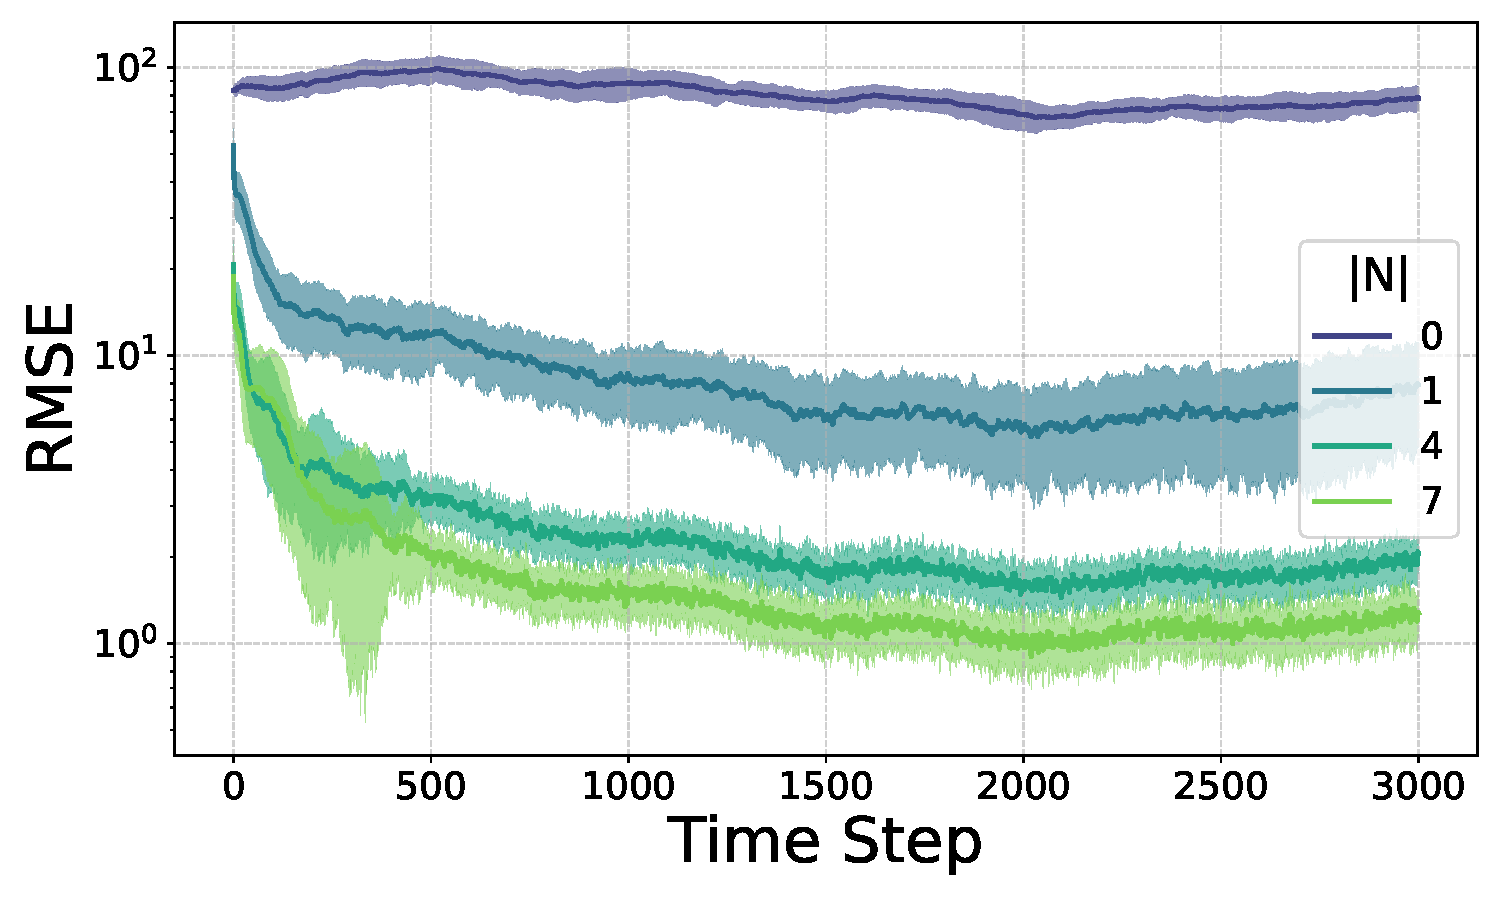
\includegraphics[width=0.49\linewidth]{figures/distributed_state_estimation/dcoss/charts/experiment1/rmse.pdf}
    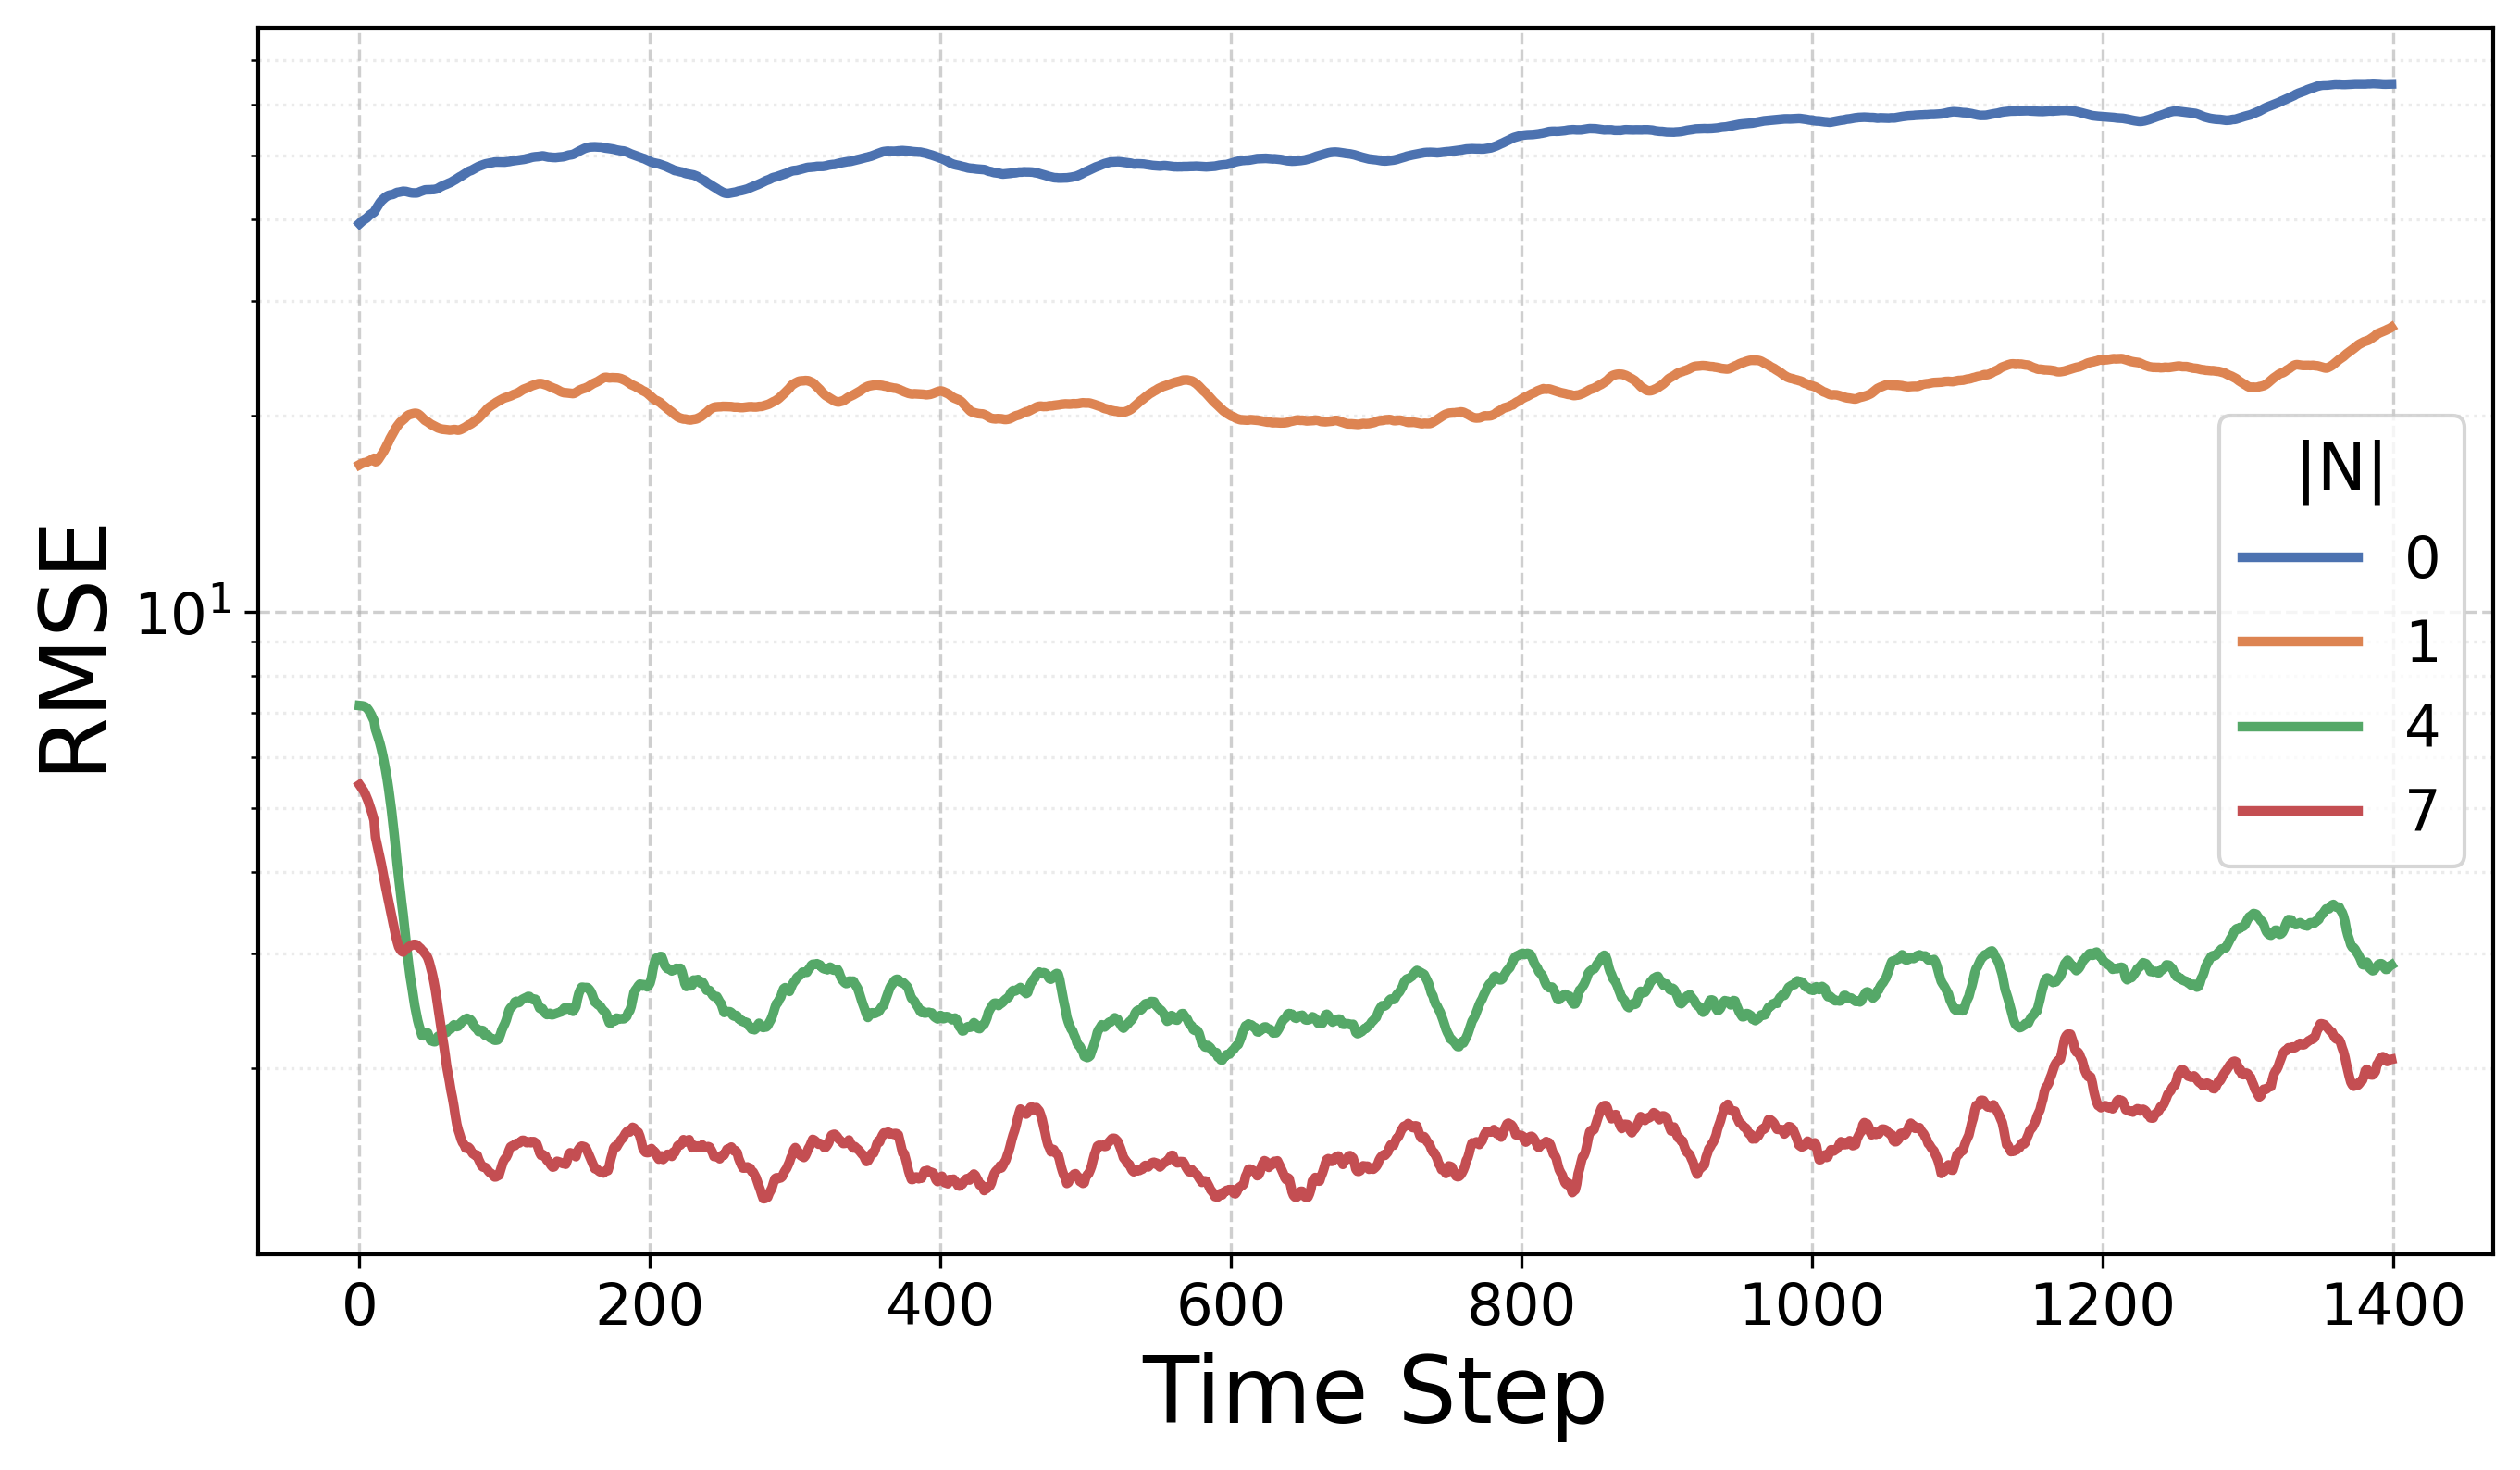
\includegraphics[width=0.49\linewidth]{figures/distributed_state_estimation/acsos/charts/experiment1/RMSE.png}
    \caption{Effect of neighborhood measurement sharing on estimation error.
    Top: single-target results averaged over $100$ random seeds.
    Bottom: multi-target results averaged over $50$ random seeds.
    The curves distinguish the number of communication neighbors; the device's own observation is also used.
    The studies use different trajectories and durations, so the plots support a qualitative comparison of the effect of cooperation.}
    \label{fig:dpf-local-rmse}
\end{figure}

The reconstructed multi-target trajectories in \Cref{fig:dpf-multi-trajectories} illustrate 
 the corresponding spatial behavior.
%
Small neighborhoods provide insufficient information 
 to recover the trajectories reliably.
%
Larger neighborhoods allow the estimates to follow the targets 
 more closely after an initial transient.
%
These results show that measurement sharing can support cooperative tracking 
 without a fusion center or particle exchange.
%
They characterize the benefit of increased information availability; 
 communication cost is not independently measured by these error curves.

\begin{figure}
    \centering
    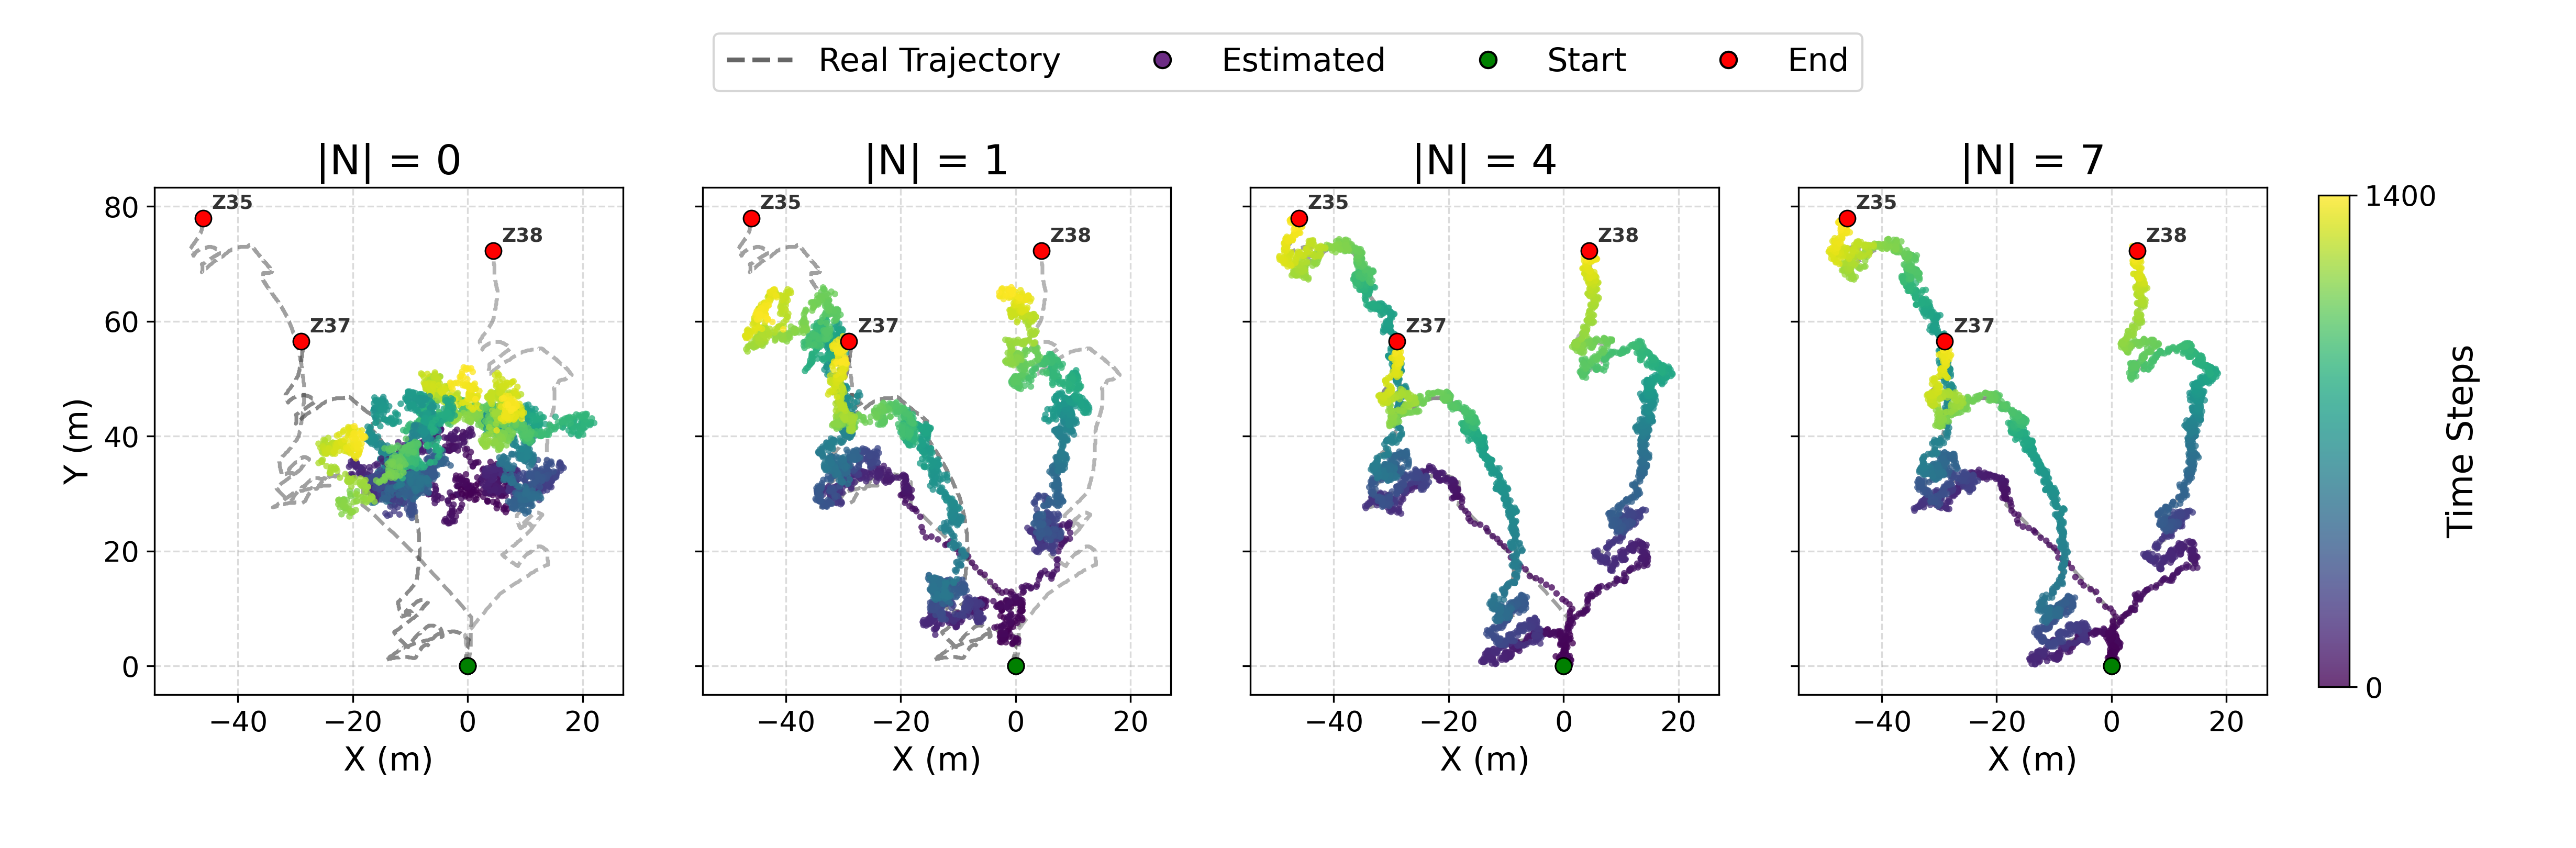
\includegraphics[width=\linewidth]{figures/distributed_state_estimation/acsos/charts/experiment1/three_zebras_by_number_of_neighbors.png}
    \caption{Reconstructed trajectories of three moving targets with different neighborhood sizes.
    Dashed lines indicate reference trajectories and colored points indicate estimates over time.
    Increasing the number of neighbors improves reconstruction through a richer set of spatial observations.}
    \label{fig:dpf-multi-trajectories}
\end{figure}

\subsection{Recovery After Fusion-Center Failure}
\label{subsec:dpf-failure-results}

The leader-based experiments remove the elected fusion device midway through a run.
%
The failure occurs at step $1500$ in the synthetic single-target case 
 and at step $700$ in the multi-target case.
%
\Cref{fig:dpf-leader-recovery} shows the estimated trajectories before 
 and after these events.
%
An initial transient accompanies the first election 
 and the start of filtering.
%
A second transient follows leader failure, 
 after which the replacement device resumes tracking.

\begin{figure}
    \centering
    \begin{minipage}{0.4\linewidth}
        \centering
        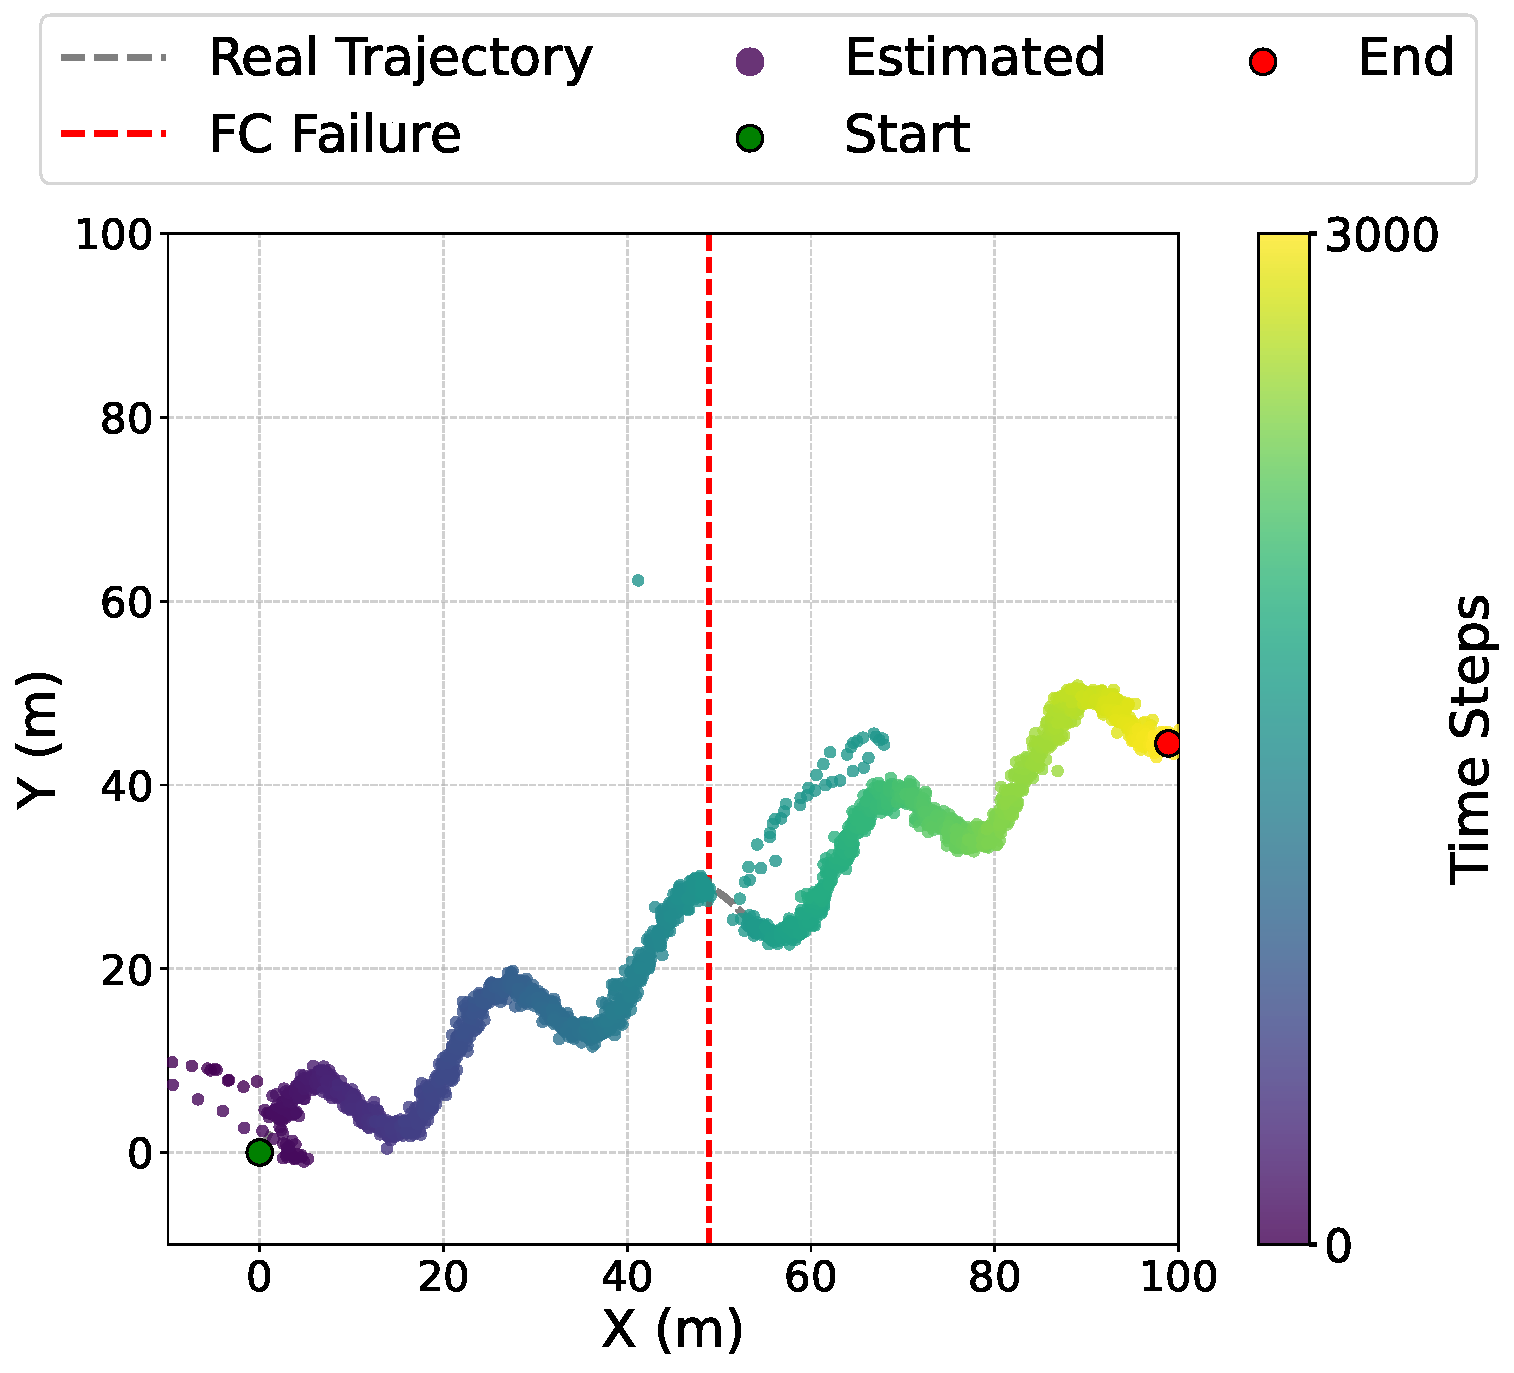
\includegraphics[width=\linewidth]{figures/distributed_state_estimation/dcoss/charts/experiment2/trajectories-fc-based.pdf}
        \par\smallskip
        (a) Single target
    \end{minipage}
    \begin{minipage}{0.4\linewidth}
        \centering
        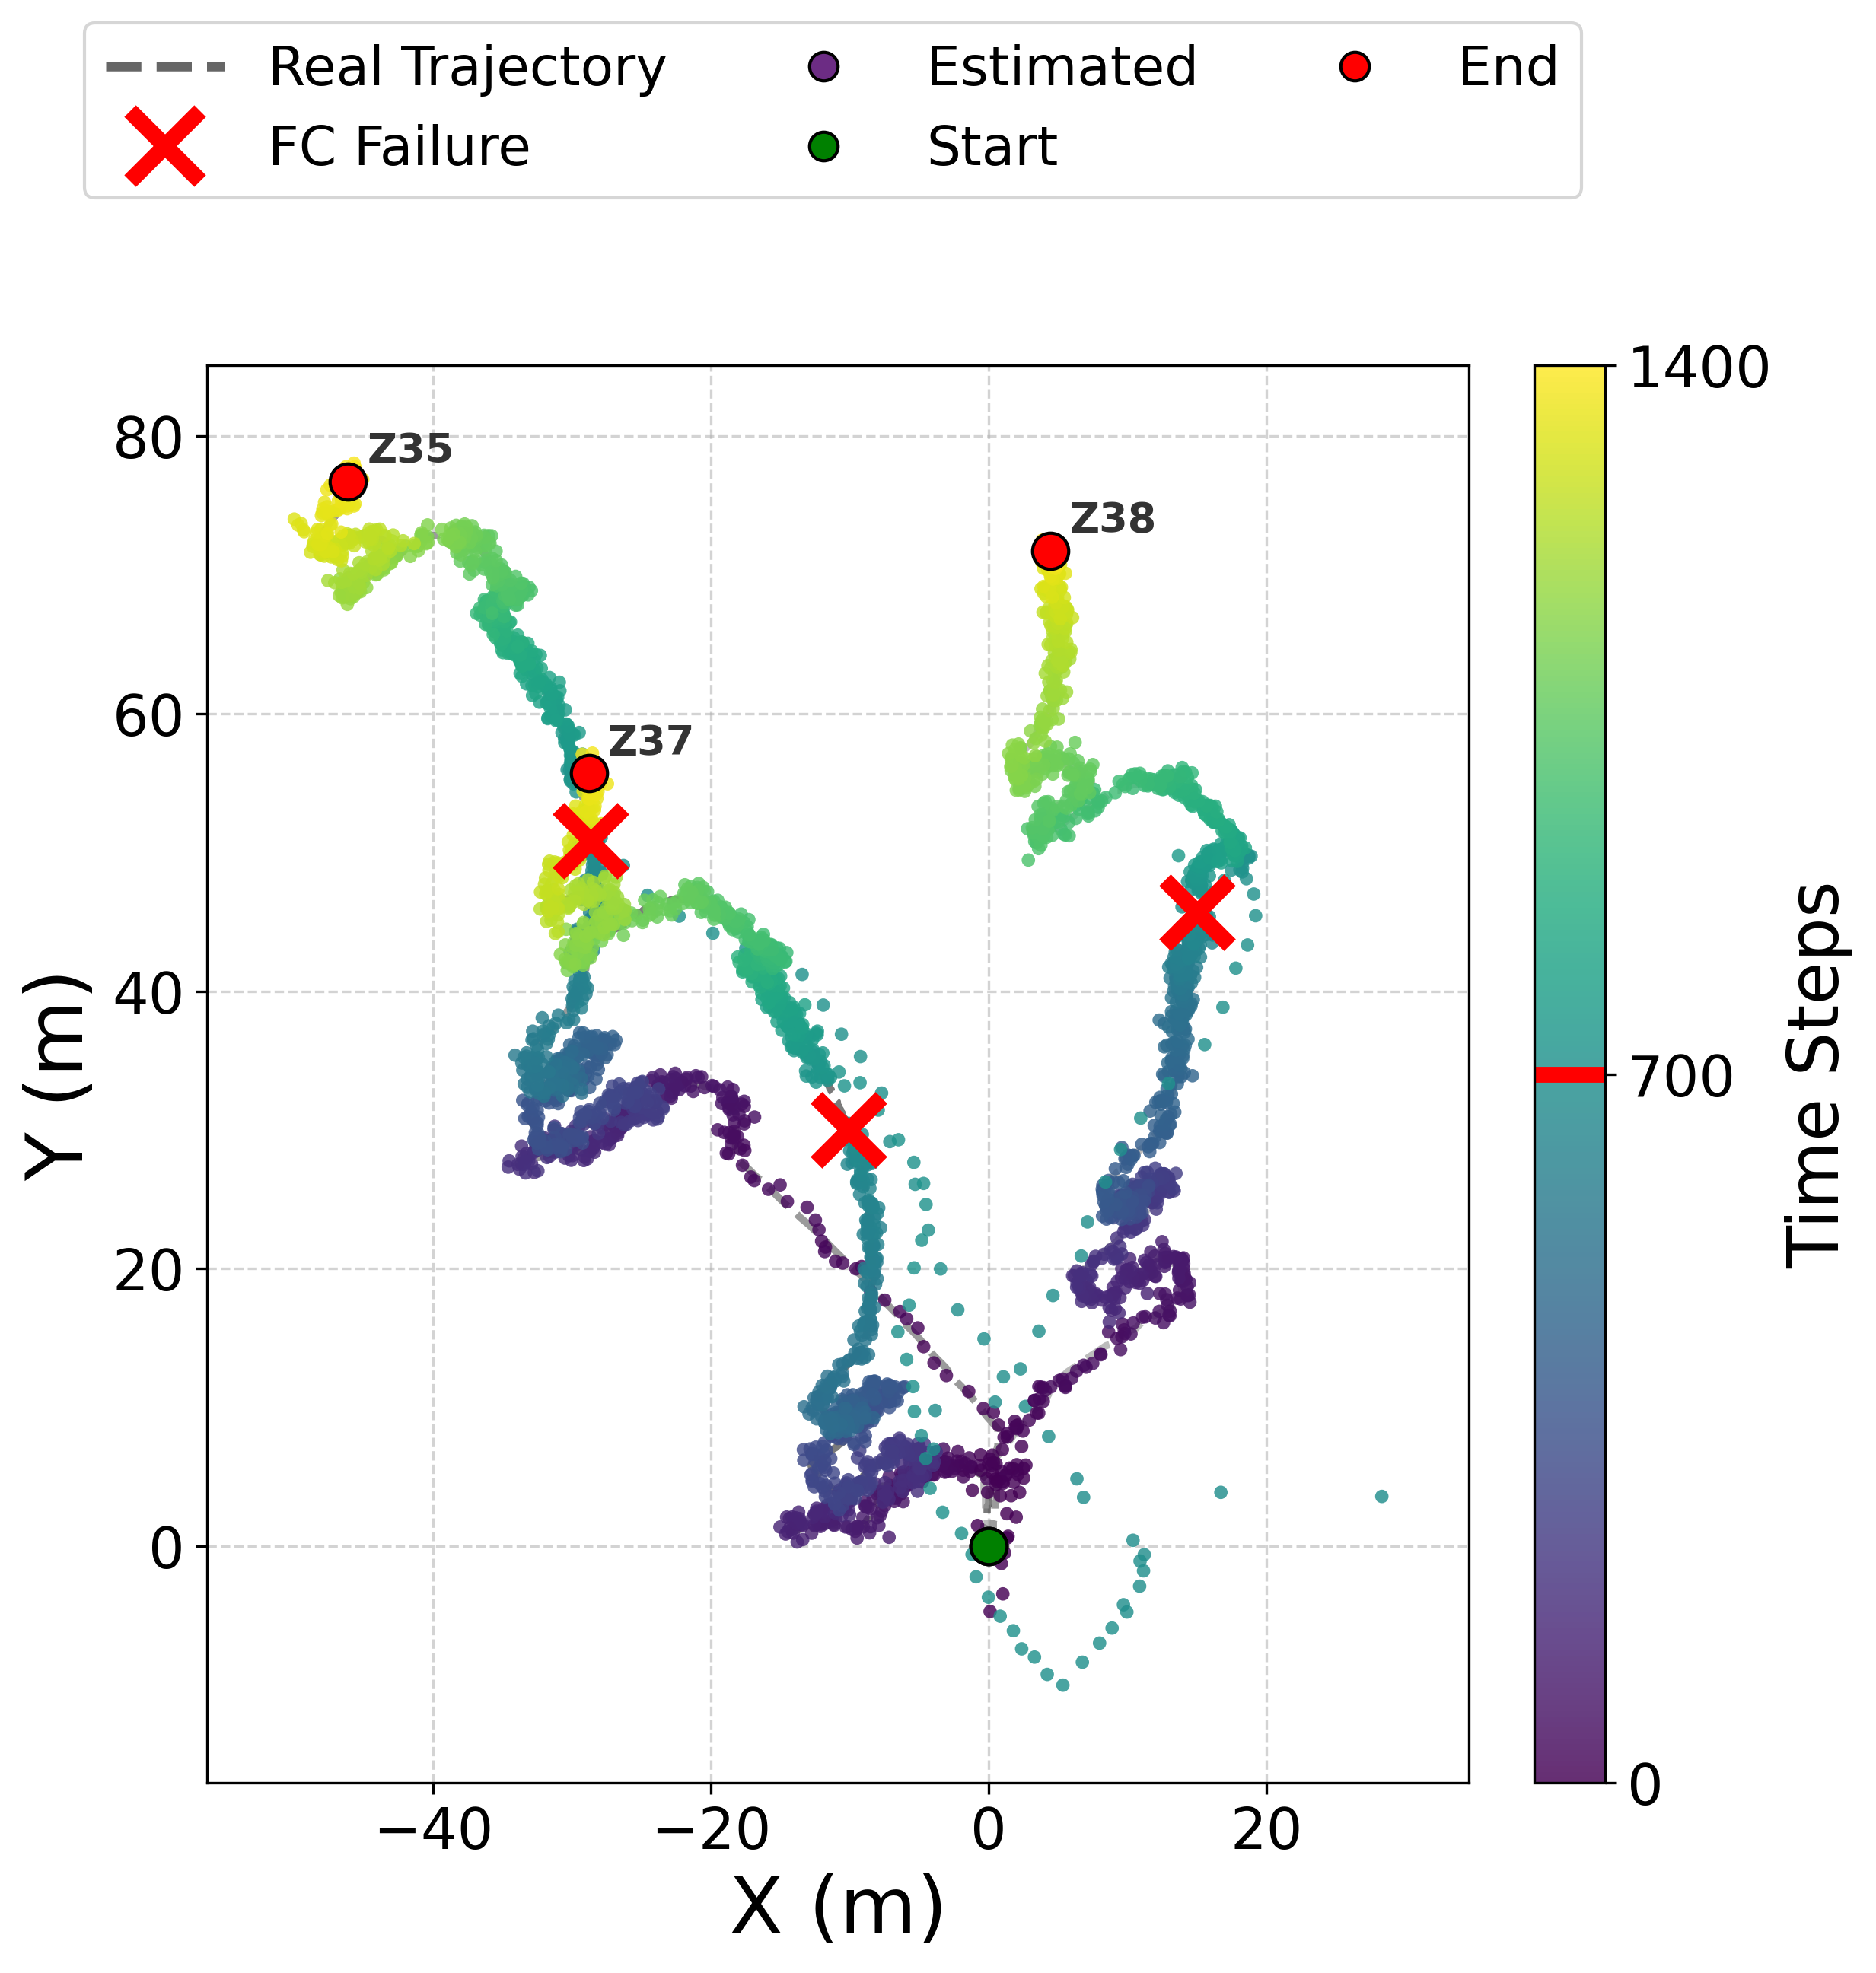
\includegraphics[width=\linewidth]{figures/distributed_state_estimation/acsos/charts/experiment2/three_zebras_fc_failure.png}
        \par\smallskip
        (b) Multiple targets
    \end{minipage}
    \caption{Tracking under failure of the elected fusion center.
    Failure is introduced at step $1500$ in the single-target run and step $700$ in the multi-target run.
    Both configurations exhibit a transient followed by resumed tracking as the aggregate coordination selects a replacement.}
    \label{fig:dpf-leader-recovery}
\end{figure}

The result demonstrates recovery 
 of the fusion role through runtime coordination.
%
The filtering procedure does not need a different architecture-specific recovery protocol 
 to identify a replacement sensor.
%
However,
 a functioning leader is still required in this configuration, 
 and its processing and collection responsibilities remain a potential bottleneck.
%
The experiment therefore supports resilience to the tested leadership loss 
 rather than a claim that fusion-based estimation has become fully decentralized.

\subsection{Mobile Sensing Infrastructure}
\label{subsec:dpf-mobility-results}

The mobile experiment combines local multi-target filtering with coordinated sensor movement.
%
Sensors preserve their relative grid-like arrangement 
 while following the estimated centroid of the targets, 
 as illustrated in \Cref{fig:dpf-mobile-sensing}.
%
Their changing positions influence subsequent observations, 
 which in turn update the estimates used for motion coordination.
%
The accompanying error plot shows that larger deviations of the sensing formation 
 from its tracking reference are associated with higher estimation RMSE.

\begin{figure}
    \centering
    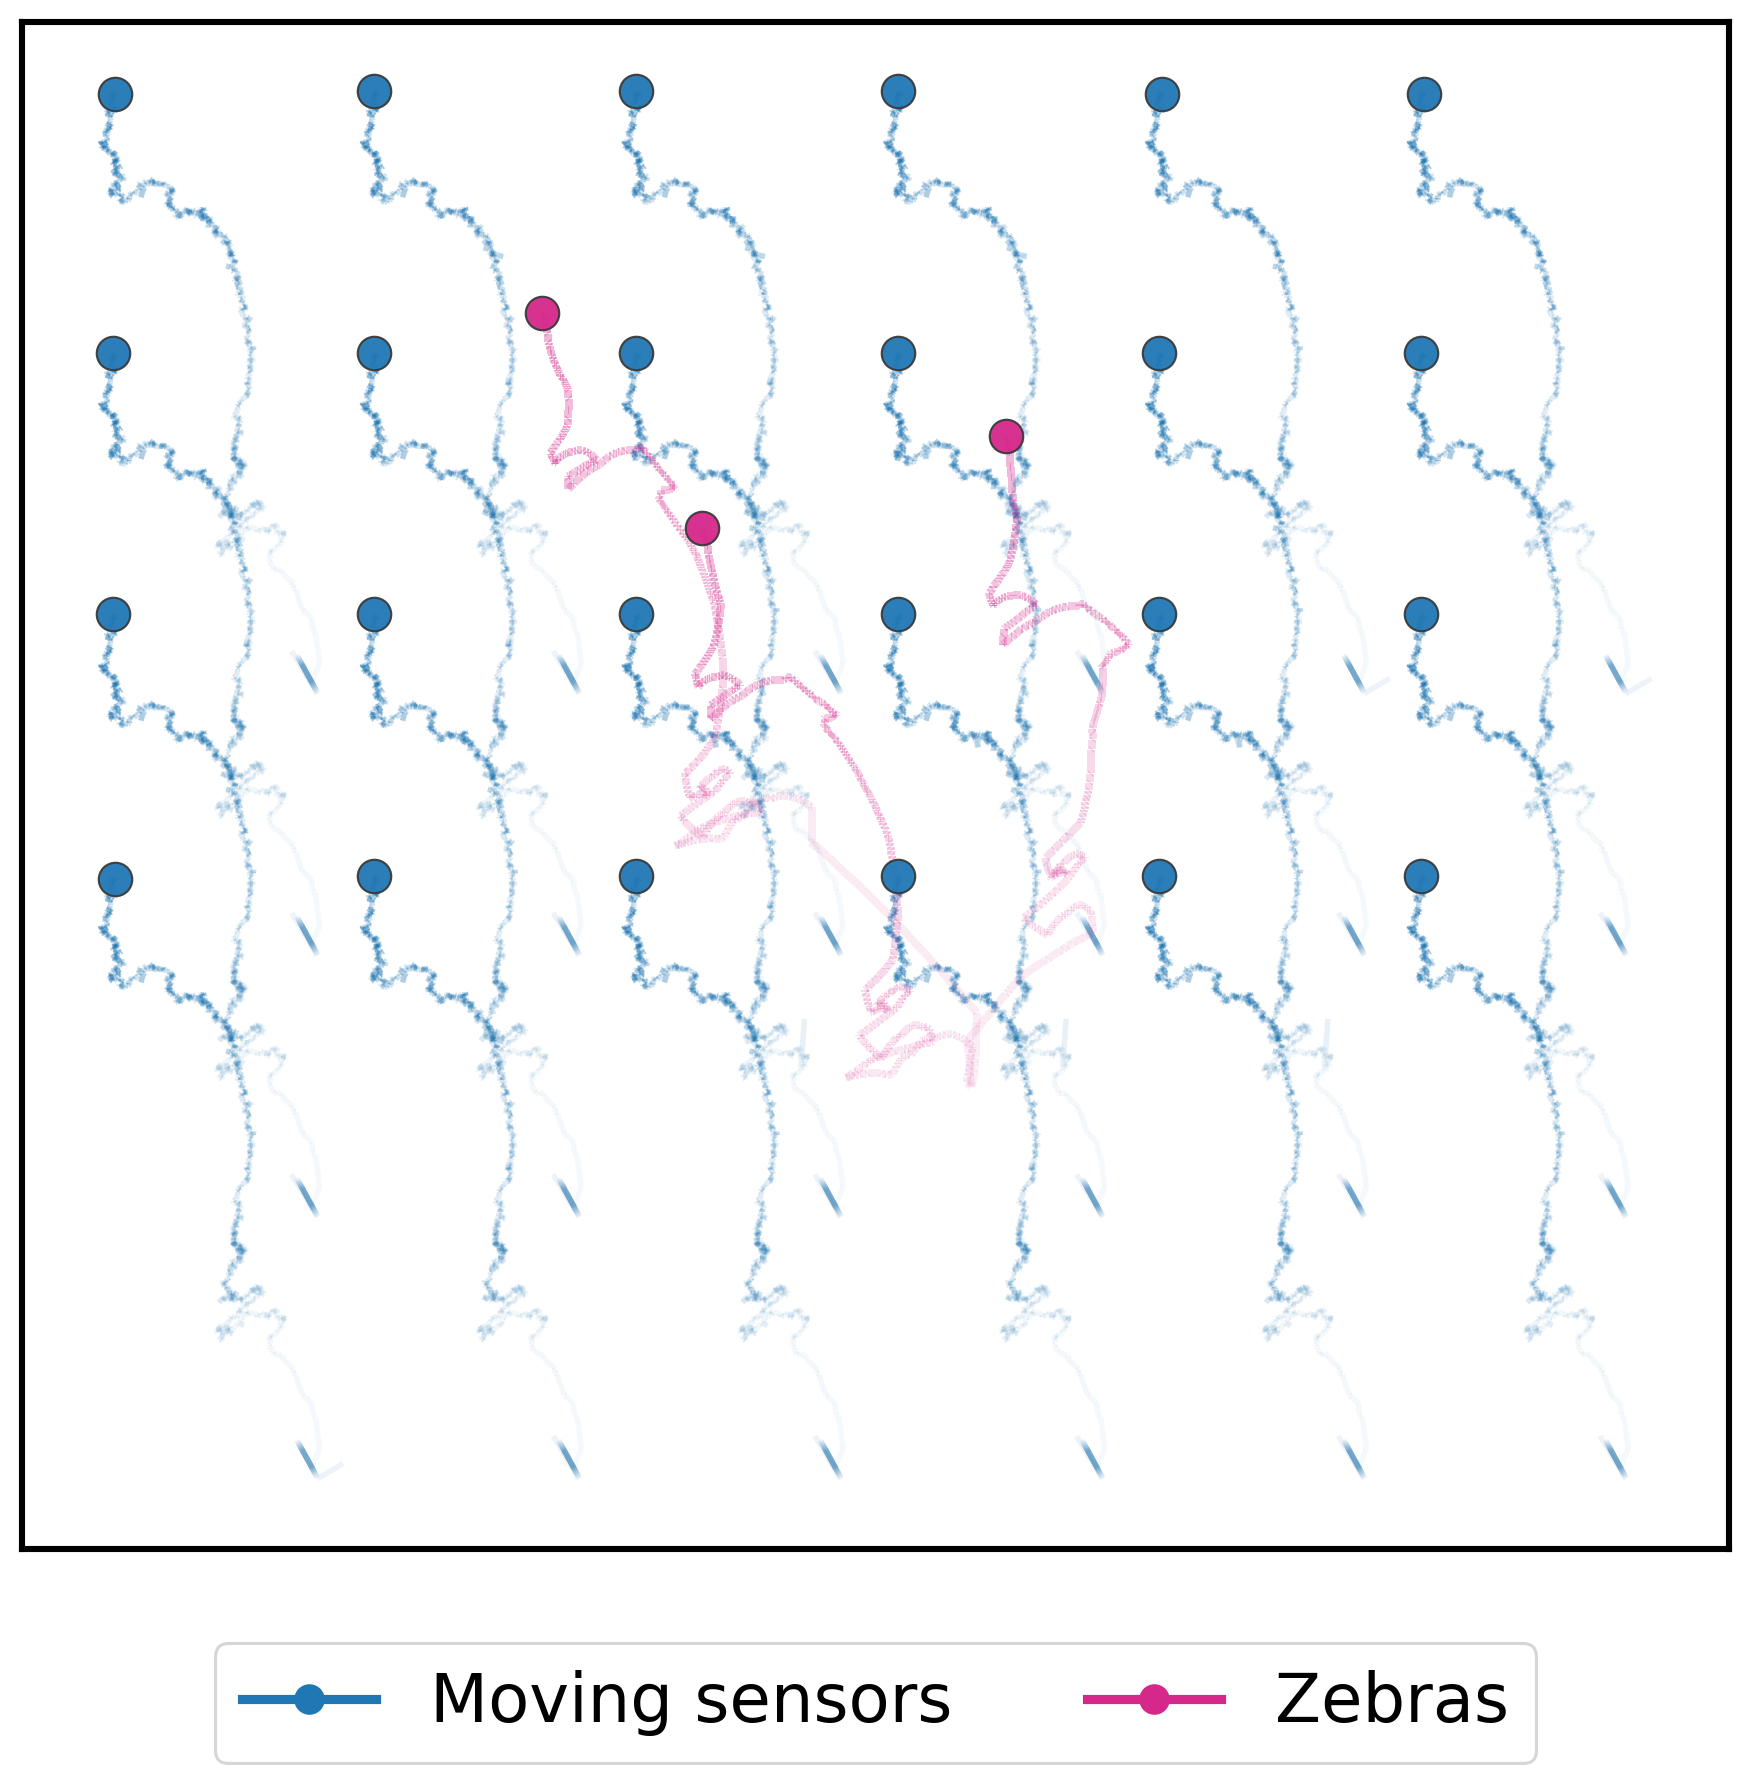
\includegraphics[width=0.4\linewidth]{figures/distributed_state_estimation/acsos/charts/AdaptiveSensorsMovement/sensors_zebras_movement.png}
    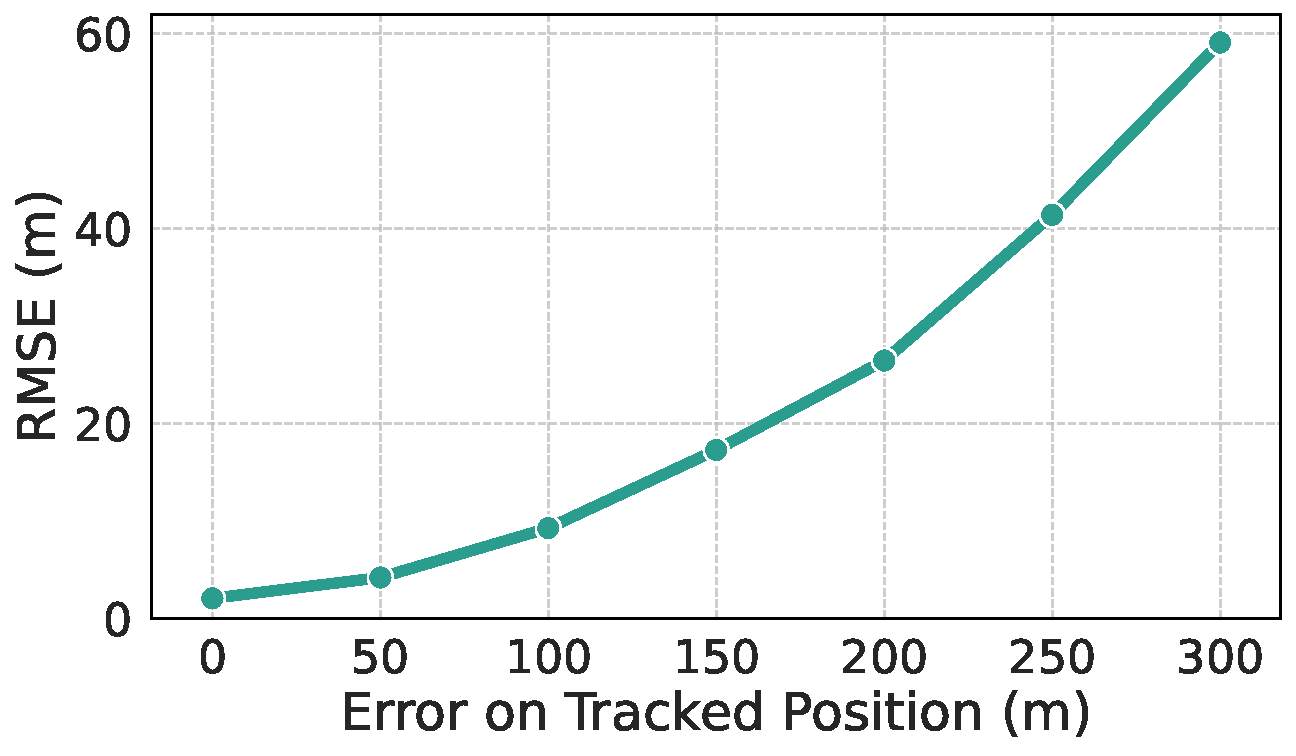
\includegraphics[width=0.49\linewidth]{figures/distributed_state_estimation/acsos/charts/AdaptiveSensorsMovement/rmse_by_error_on_position.pdf}
    \caption{Coupling between sensing geometry and estimation.
    Top: sensor and target trajectories, with markers indicating final positions; sensors preserve a grid-like formation while following the moving targets.
    Bottom: estimation RMSE as a function of the moving sensors' positional tracking error.
    Less accurate spatial tracking is associated with less accurate state estimation.}
    \label{fig:dpf-mobile-sensing}
\end{figure}

This experiment illustrates adaptation of the sensing infrastructure to the observed process.
The motion coordinator organizes the formation while the filters continue to operate locally, demonstrating that different responsibilities can use different coordination structures within the same aggregate program.
The experiment does not learn the movement policy or establish an optimal sensing arrangement; it shows how an explicit coordination strategy can be coupled to distributed estimation.

\section{Discussion and Future Directions}
\label{sec:dpf-discussion}

The common result across these experiments is that the organization of cooperation 
 influences both the availability and the usefulness of information.
%
Neighborhood sharing changes the evidence entering each filter, 
 leader election changes where fusion occurs,
 and sensor movement changes the geometry from which observations are generated.
%
\gls{AC} expresses these choices using a common coordination model, 
 allowing the estimator and its distributed organization to be considered separately 
 while retaining their operational interaction.

Several limits qualify the findings.
%
The studies evaluate a small, 
 fixed sensor population and a limited number of targets, 
 so they do not establish scaling behavior as the network grows.
%
They also do not provide a systematic comparison against alternative \gls{DPF} algorithms 
 or a measured characterization of communication and energy costs.
%
Target identifiers simplify measurement association, 
 and simulated radio observations do not capture the full variability of physical sensing.
%
Finally, 
 successful recovery in the evaluated failures does not constitute a proof of convergence 
 or self-stabilization of the complete probabilistic estimator.
%
Such properties require analysis beyond the coordination behavior 
 of its constituent aggregate operators.

Future work can investigate adaptive sensing regions, 
 heterogeneous observation models, delayed measurements, and larger target populations.
%
In particular, 
 selecting the spatial scope of cooperation according to uncertainty
 or measurement relevance could connect estimation quality to communication and computational budgets.
%
These questions extend the same engineering perspective developed here: 
 the structure of cooperation should adapt to the information required by the task 
 and to the resources available in the collective.

For cooperative learning, 
 distributed estimates could provide observations to decision policies or inputs to predictive models,
 while learned models could inform motion prediction, sensor selection, or coordination.
%
These integrations have not been evaluated in the presented studies.
%
The contribution established here is the coordination 
 of collective state estimation under partial observations and changing responsibilities, 
 complementing the following investigation of how devices organize collaboration to learn from distributed data.